%\chapter{開発プロセス}
\section{第2サイクル}
第2サイクルは中間発表会用のポスターレビューから中間発表会までとした。本サイクルでは第1サイクルで課題として残ったユーザストーリの流れを改善すること、第 1 回フィールドワークであげられた観光中に撮影した写真が整理されていないという課題を解決すべき問題として定義した。本サイクルでは2つの問題に同時で取り組んでいった。\\
1つ目のユーザストーリの流れを改善することに対しては、中間成果発表会まで残り1 週間を切っていたため新たな機能を追加して修正するのは間に合わないと判断し、第1サイクルで実装していた部分の情報の見せ方を改善する方針で議論を進めた。具体的に修正した内容を表5.2に、実装した画面は図5.2(a)に示す。2つ目の観光中に撮影した写真が整理されていないという問題への解決アプローチとしてフォトストーリーという機能を考案した。これはユーザが撮影した写真と移動した経路を表示したマップが図5.2(b)のような紀行*1 となり、木古内町観光をよりリアルに振り返れる仕組みである。当時考案していたフォトストーリーのユーザストーリの流れとフォトストーリーに対するレビュー内容を以下に示す。\\なお、本サイクルではアプリ全体のユーザストーリの流れは多少改善されたがまだベストな状態とは言えなかった。フォトストーリに関しては、ユーザが写真を撮るという行為にワクワクする付加価値が必要という課題が残った。

\begin{table}[htb]
\centering
\addtocounter{table}{+1}
\caption{第1サイクルから第2サイクルへの変化}
  \begin{tabular}{|l|l|} \hline
    改正前&改正後  \\ \hline 
    食べる・見る・買うのカテゴリ別にピンを表示 & カテゴリは変えずに写真の一覧を表示 \\  \hline
    お店の詳細情報としてWeb ページを表示 &詳細情報の表示方法は我々で作成した画面構成を用いる\\ \hline
    マップ画面が最初に表示 & カテゴリ別になった写真一覧を最初に表示\\ \hline
    目的地までのルートのみ表示 & ルートの他に距離と徒歩及び車での所要時間を表示 \\ \hline
  \end{tabular} 
\end{table}

\begin{figure}[htbp]
  \begin{center}
    \begin{tabular}{c}

      % 1
      \begin{minipage}{0.33\hsize}
        \begin{center}
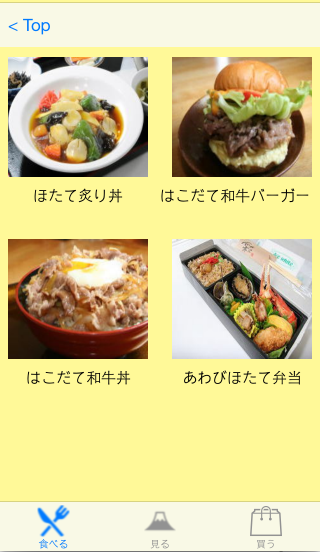
\includegraphics[width=4cm, bb=0 0 320 552]{5.4_category.png}
          \hspace{1cm} [1]観光スポットの紹介
        \end{center}
      \end{minipage}

      % 2
      \begin{minipage}{0.33\hsize}
        \begin{center}
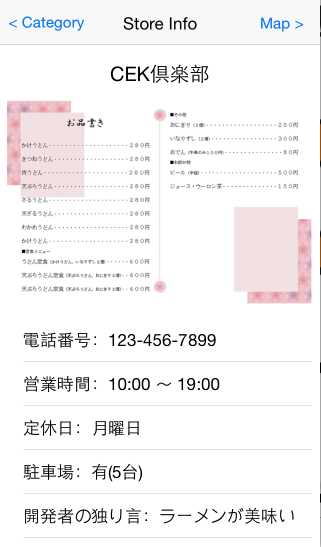
\includegraphics[width=4cm, bb=0 0 321 547]{5.4_detail.png}
          \hspace{1cm} [2]詳細情報の表示
        \end{center}
      \end{minipage}

      % 3
      \begin{minipage}{0.33\hsize}
        \begin{center}
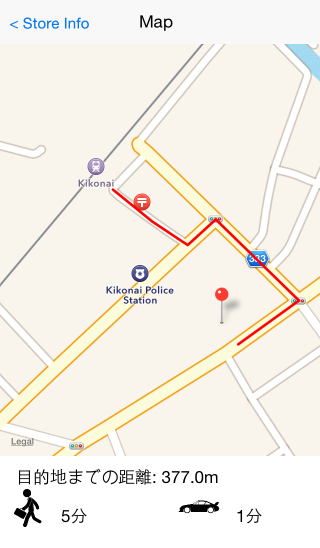
\includegraphics[width=4cm, bb=0 0 320 548]{5.4_route.png}
          \hspace{1cm} [3]ルート案内
        \end{center}
      \end{minipage}

    \end{tabular}
    \caption{(a)第2サイクルの完成画面}
    \label{fig:lena}
  \end{center}
\end{figure}

\begin{description}
 \item[フォトストーリーの説明]\mbox{}
 \begin{enumerate}
 \item フォトストーリーを使用することでどのような紀行が出来上がるのかのサンプル動画を見る。この動画にはフォトストーリーの操作説明及び木古内町の魅力が内容として含まれているため、操作方法だけでなく木古内の魅力も知ることができる。
  \item 観光中に撮影した写真をアプリ内に保存。
 \item 撮影した写真の一覧が表示され、ユーザが写真を任意のカテゴリ別に分けることができる。
 \item 加工ボタンを押すとユーザが撮影した写真と移動した経路を表示したマップが紀行として画面に表示される。
 \item フォトストーリーを使用してユーザの思い出話によるコミュニケーションが促進される。
\end{enumerate}
\item[フォトストーリーへのレビュー内容]\mbox{}
 \begin{itemize}
 \item 木古内町の歴史に関する情報を表示する機能が欲しい
 \item 図5.2(b)に対して、1 つの画面に写真が2 枚もあると分かりにくい
 \item 写真を撮りたくなるトリガーがないため、フォトストーリの存在が危うい
 \item 時系列での説明をされると聞いている側は辛くなってしまう。2,3枚ほどのダイジェストの方が良い。
 \item フォトストーリーを実装するのであれば、誰が写真を撮るのかを考えてUI設計を行うこと。スマートフォンに使い慣れた若い人と大人と子供ではそれぞれUIが違ってくる。
 \item 案内だけに留まらずに思い出に着眼したことは良い。今後の掘り下げ方で何倍にも良いものになる可能性がある。
 \end{itemize}
\end{description}

\begin{figure}[htbp]
 \begin{center}
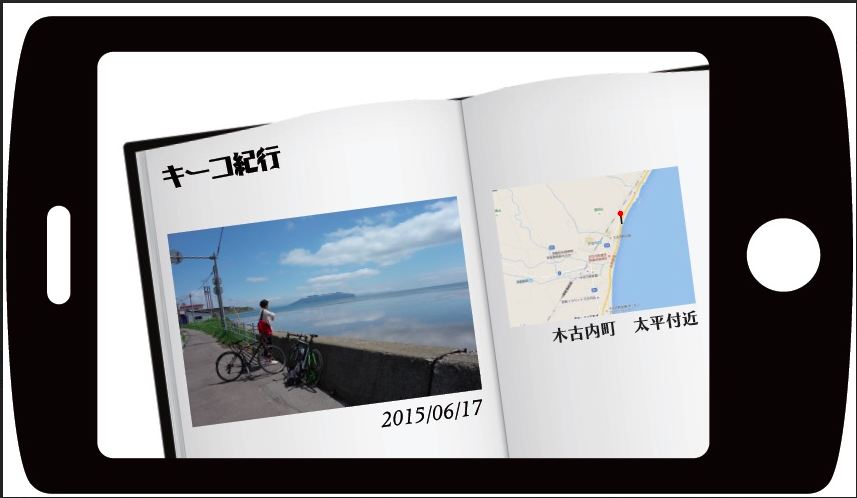
\includegraphics[width=9cm, bb=0 0 857 498]{5.1_kikou.png}
 \end{center}
\addtocounter{figure}{-1}
 \caption{(b)紀行の画面イメージ}
 \label{fig:one}
\end{figure}
\bunseki{岩見建汰}